\subchapter{Measure boot time - Software solution}{Objective: measure
boot time with software only solutions}

During this lab, we will use techniques to measure boot time using only
software solutions.

\section{Timing messages on the serial console}

Let's use \code{grabserial} to time all the messages received in the
serial console, from the first stage bootloader to launching the final
application:

\begin{verbatim}
sudo apt install grabserial
\end{verbatim}

We are now ready to time the messages in the serial console. First, exit
from Picocom (\code{[Ctrl][a] [Ctrl][x]}). Then, power off your board,
remove its USB power supply and run:

\begin{verbatim}
grabserial -d /dev/ttyUSB0 -t -e 30
\end{verbatim}

\begin{itemize}
\item \code{-t} Displays the time when the first character of each line
was received.
\item \code{-e} Specifies the {\bf e}nd time when \code{grabserial}
will exit.
\end{itemize}

Now, plug in the power cable and see the console messages with their
timing information:

\begin{verbatim}
[0.000001 0.000001]
[0.000838 0.000838] U-Boot SPL 2022.04 (Apr 15 2022 - 16:20:37 +0200)
[0.004477 0.004477] Trying to boot from MMC1
[0.602845 0.598369]
[0.602970 0.000125]
[0.603040 0.000069] U-Boot 2022.04 (Apr 15 2022 - 16:20:37 +0200)
...
\end{verbatim}

As you can see, the time to start U-Boot SPL can be neglected. We can
use the \code{U-Boot SPL} string as a reference point for timing. This way,
we don't have to power off the board every time we wish to make a
measurement. Resetting the board will be sufficient.

So, let's run \code{grabserial} again:

\begin{verbatim}
grabserial -d /dev/ttyUSB0 -m "U-Boot SPL" -t -e 30
\end{verbatim}

\section{Timing the execution of the application}

Bootlin prepared a patch to \code{ffmpeg} to issue a message in its logs
after decoding and displaying the first frame. Let's instruct Buildroot
to apply it!

\begin{verbatim}
mkdir -p board/beaglecam/patches/ffmpeg/
cp ../data/0001-ffmpeg-log-notification-after-first-frame.patch \
   board/beaglecam/patches/ffmpeg/
\end{verbatim}

Then, tell Buildroot to look for patches in this directory, by adding
\code{board/beaglecam/patches} to the
\code{BR2_GLOBAL_PATCH_DIR} configuration setting (through \code{make
menuconfig} or by directly editing the \code{.config} file.

Then, rebuild \code{ffmpeg}:

\begin{verbatim}
make ffmpeg-dirclean
make
\end{verbatim}

Note that \code{make ffmpeg-rebuild} wouldn't be sufficient to apply a
newly added patch.

Let's add something else before updating the root filesystem image...

\section{Timing the launching of the application}

To measure the time the application takes to load and execute, it's also
very useful to time the instant when the application is started.

So, let's also modify \code{board/beaglecam/rootfs-overlay/etc/init.d/S50playvideo}
to add the below line before running \code{ffmpeg}:

\begin{verbatim}
echo "Starting ffmpeg"
\end{verbatim}

Now we can update the root filesystem image:

\begin{verbatim}
make
\end{verbatim}

After reflashing the SD card, reset the board and check that you are
getting the new message. You can now measure the time between starting
\code{ffmpeg} and finishing processing the first frame.

Before running \code{grabserial} again, let's create the {\code
$HOME/logs/} in which we will store copies of the command's output:

\begin{verbatim}
mkdir ~/logs/
\end{verbatim}

Thanks to the last message, we can now stop \code{grabserial} when it's
received, replacing the \code{-e} argument:

\begin{verbatim}
grabserial -d /dev/ttyUSB0 -m "U-Boot SPL" -t -q "First frame decoded" \
           -o ~/logs/initial.log
\end{verbatim}

We now have a complete measurement of the initial boot time of the
system. We are going to write down the key figures, but it's always
useful to keep the full log each of our experiments. This is very often
useful to compare experiments, double check some measurements that
are surprising and could have been copied in a wrong way, and
investigate some differences between two different runs.

\section{Initial measurements}

Now, run the test 3 times and using LibreOffice Calc, fill the \code{Run 1},
\code{Run 2} and \code{Run 3} columns in the table in the
\code{~/boot-time-labs/results/initial.ods} spreadsheet. The averages and standard
deviations of the measurements will be computed automatically.

Here's the kind of results you should get after filling the table:

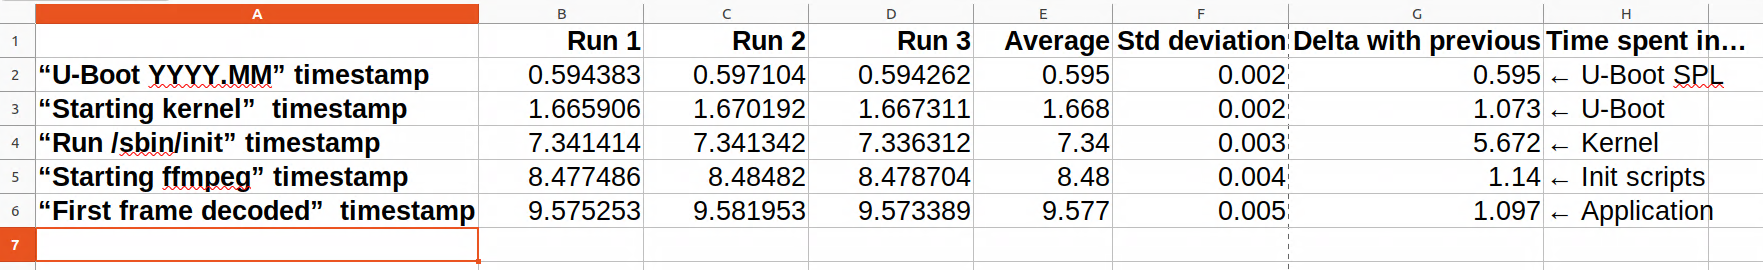
\includegraphics[width=\textwidth]{labs/boot-time-software-measurement/initial.png}

